\documentclass{beamer}[10]

\usepackage{graphicx}
\usepackage{xcolor}
\usepackage{tabto}
%\usepackage{beamerthemesplit}
\usepackage{tikz}
\usepackage{cancel}
\usepackage{verbatim}
\usepackage{fancybox}
\usepackage{enumerate}
\usepackage{amsmath,amssymb,amsthm,textcomp,mathtools}
\usepackage[super]{nth}
\usepackage[amssymb]{SIunits}
\usepackage{booktabs}
\usepackage{cancel}
\usepackage{bm}
\usepackage[utf8]{inputenc}
\usepackage{tabularx}
\usepackage{ragged2e}
\newcolumntype{Y}{ >{\RaggedRight\arraybackslash}X}
\usetikzlibrary{arrows,shapes}
\newcommand\T{\rule{0pt}{2.6ex}}
\newcommand\B{\rule[-1.2ex]{0pt}{0pt}}
\definecolor{UUcrimson}{RGB}{204,0,0}
\mode<presentation>
{ \usetheme{default}
  \usecolortheme[named=UUcrimson]{structure}
  \useinnertheme{circles}
  \setbeamercovered{transparent}
  \setbeamertemplate{blocks}[rounded]
  \usefonttheme[onlymath]{serif}
  \setbeamertemplate{navigation symbols}{}
  \setbeamertemplate{footline}[page number]
  \setbeamertemplate{navigation symbols}{}
  \setbeamercolor{section in toc}{fg=black,bg=white}
  \setbeamercolor{alerted text}{fg=UUcrimson!80!gray}
  \setbeamercolor*{palette primary}{fg=white,bg=UUcrimson}
  \setbeamercolor*{palette secondary}{fg=UUcrimson!70!black,bg=gray!15!white}
  \setbeamercolor*{palette tertiary}{bg=UUcrimson!80!black,fg=gray!10!white}
  \setbeamercolor*{palette quaternary}{fg=UUcrimson,bg=gray!5!white}
  \setbeamercolor*{palette sidebar primary}{fg=UUcrimson!10!black}
  \setbeamercolor*{palette sidebar secondary}{fg=white}
  \setbeamercolor*{palette sidebar tertiary}{fg=UUcrimson!50!black}
  \setbeamercolor*{palette sidebar quaternary}{fg=gray!10!white}
  \setbeamercolor{titlelike}{parent=palette primary,fg=white}
  \setbeamercolor{frametitle}{bg=UUcrimson}
  \setbeamercolor{frametitle right}{bg=UUcrimson}
  \setbeamercolor*{separation line}{}
  \setbeamercolor*{fine separation line}{}
}

\usetikzlibrary{backgrounds}
\makeatletter
\tikzstyle{every picture}+=[remember picture]
\tikzset{%
  fancy quotes/.style={
    text width=\fq@width pt,
    align=justify,
    inner sep=1em,
    anchor=north west,
    minimum width=\linewidth,
    font=\itshape
  },
  fancy quotes width/.initial={.8\linewidth},
  fancy quotes marks/.style={
    scale=8,
    text=white,
    inner sep=0pt,
  },
  fancy quotes opening/.style={
    fancy quotes marks,
  },
  fancy quotes closing/.style={
    fancy quotes marks,
  },
  fancy quotes background/.style={
    show background rectangle,
    inner frame xsep=0pt,
    background rectangle/.style={
      fill=gray!25,
      rounded corners,
    },
  }
}
\newenvironment{fancyquotes}[1][]{%
\noindent
\tikzpicture[fancy quotes background]
\node[fancy quotes opening,anchor=north west] (fq@ul) at (0,0) {``};
\tikz@scan@one@point\pgfutil@firstofone(fq@ul.east)
\pgfmathsetmacro{\fq@width}{\linewidth - 2*\pgf@x}
\node[fancy quotes,#1] (fq@txt) at (fq@ul.north west) \bgroup}
{\egroup;
\node[overlay,fancy quotes closing,anchor=east] at (fq@txt.south east) {''};
\endtikzpicture}
\makeatother


\usetikzlibrary{backgrounds}
\makeatletter
\tikzstyle{every picture}+=[remember picture]
\tikzset{%
  fancy defs/.style={
    text width=\fq@width pt,
    align=justify,
    inner sep=0.25em,
    anchor=north west,
    minimum width=\linewidth,
    font=\itshape
  },
  fancy defs width/.initial={.8\linewidth},
  fancy defs marks/.style={
    scale=8,
    text=white,
    inner sep=0pt,
  },
  fancy defs opening/.style={
    fancy defs marks,
  },
  fancy defs closing/.style={
    fancy defs marks,
  },
  fancy defs background/.style={
    show background rectangle,
    inner frame xsep=0pt,
    background rectangle/.style={
      fill=gray!25,
      rounded corners,
    },
  }
}
\newenvironment{fancydefs}[1][]{%
\noindent
\tikzpicture[fancy defs background]
\node[fancy defs opening,anchor=north west] (fq@ul) at (0,0) {};
\tikz@scan@one@point\pgfutil@firstofone(fq@ul.east)
\pgfmathsetmacro{\fq@width}{\linewidth - 2*\pgf@x}
\node[fancy defs,#1] (fq@txt) at (fq@ul.north west) \bgroup}
{\egroup;
\node[overlay,fancy defs closing,anchor=east] at (fq@txt.south east) {};
\endtikzpicture}
\makeatother
\usepackage{scalerel}[2014/03/10]
\usepackage{stackengine}
\usepackage{empheq}
\newcommand*\widefbox[1]{\fbox{\hspace{0.5em}#1\hspace{0.5em}}}

\newcommand\reallywidetilde[1]{\ThisStyle{%
  \setbox0=\hbox{$\SavedStyle#1$}%
  \stackengine{-.1\LMpt}{$\SavedStyle#1$}{%
    \stretchto{\scaleto{\SavedStyle\mkern.2mu\sim}{.5467\wd0}}{.4\ht0}%
%    .2mu is the kern imbalance when clipping white space
%    .5467++++ is \ht/[kerned \wd] aspect ratio for \sim glyph
  }{O}{c}{F}{T}{S}%
}}
\usepackage{media9}

\logo{
\includegraphics[width=0.75cm]{logo.jpg}}
\author[Gibbs]{Dr. Jeremy A. Gibbs}
\institute{Department of Mechanical Engineering\\University of Utah}
\date{Spring 2017}
\title{Environmental Fluid Dynamics: Lecture 10}
% colors
\definecolor{colororange}{HTML}{E65100} % orange
\definecolor{colordgray}{HTML}{795548} % dark gray for note
\definecolor{colorhgray}{HTML}{212121} % heavy dark gray for normal text
\definecolor{colorgreen}{HTML}{009688} % green
\definecolor{colorwhite}{HTML}{FFFFFF} % background white
\definecolor{colorlgray}{HTML}{F5F3EE} % background light gray
\definecolor{colorblue}{HTML}{0277BB} % blue
\definecolor{colorred}{HTML}{CC0000} % red
\usepackage{esvect}
\newcommand{\fontsizeone}{1.9em}
\setbeamertemplate{caption}{\raggedright\insertcaption\par}
\newcommand{\framecard}[2][colorgreen]{
  {\setbeamercolor{background canvas}{bg=#1}
    \begin{frame}[plain]
    \vfill
    \begin{center}
     {#2}
    \end{center}
    \vfill
    \end{frame}
  }
}
\begin{document}

%----------------------------------------------------------------------------------------
%	TITLE & TOC SLIDES
%----------------------------------------------------------------------------------------

\begin{frame} 
  \titlepage
\end{frame}

%------------------------------------------------

\begin{frame}
\frametitle{Overview}
\tableofcontents
\end{frame}

%------------------------------------------------
\section{Atmospheric Dynamics: Basic Equations} %
%------------------------------------------------
\subsection{Conservation of Momentum, continued}
%------------------------------------------------
\framecard[colorred]{{\color{white}\Huge Atmospheric Dynamics:\\~\\Conservation of Momentum,\\~\\continued}}

%------------------------------------------------
\begin{frame}{Conservation of Momentum: Rotating Coordinate System}
\begin{itemize}
	\item Apparent forces (centrifugal, Coriolis) will automatically appear when we write Newton's \nth{2} Law in a form appropriate for a rotating reference frame.
	\item Consider a Cartesian coordinate system $x^\prime$, $y^\prime$, and $z^\prime$ rotating with angular velocity $\vv{\Omega}$. 
	\item Let $\hat i^\prime$, $\hat j^\prime$, $\hat k^\prime$ be unit vectors in the $x^\prime$, $y^\prime$, and $z^\prime$ directions, respectively (these vectors rotate with the coordinate system).
\end{itemize}
\end{frame}
%------------------------------------------------
\begin{frame}{Conservation of Momentum: Rotating Coordinate System}
\begin{itemize}
	\item Consider some arbitrary vector $\vv{A}$ that is observed in an inertial reference frame.
	\item Even though $\vv{A}$ is observed in a non-rotating reference frame, it can be decomposed into components in a rotating coordinate system:
	$$\vv{A} = A_x^\prime \hat{i}^\prime + A_y^\prime \hat{j}^\prime + A_z^\prime \hat{k}^\prime$$
	where
	\begin{align*}
		A_x^\prime &= \hat{i}^\prime \cdot \vv{A}\\
		A_y^\prime &= \hat{j}^\prime \cdot \vv{A}\\
		A_z^\prime &= \hat{k}^\prime \cdot \vv{A}
	\end{align*}
\end{itemize}
\end{frame}
%------------------------------------------------
\begin{frame}{Conservation of Momentum: Rotating Coordinate System}
\begin{itemize}
	\item The total derivative of $\vv{A}$ as observed in the inertial reference frame is (where subscript $a$ means absolute, or inertial):
	\begin{align*}
	\frac{D_a\vv{A}}{Dt} &= \frac{D_a}{Dt}\left( A_x^\prime \hat{i}^\prime + A_y^\prime \hat{j}^\prime + A_z^\prime \hat{k}^\prime\right)\\
	&= \underbrace{\hat{i}^\prime \frac{D_aA_x^\prime}{Dt} + \hat{j}^\prime \frac{D_aA_y^\prime}{Dt} + \hat{k}^\prime \frac{D_aA_z^\prime}{Dt}}_{\text{$D\vv{A}/Dt$ observed in rotating ref frame}} \\&+ A_x^\prime \frac{D_a \hat{i}^\prime}{Dt} + A_y^\prime \frac{D_a \hat{j}^\prime}{Dt} + A_z^\prime \frac{D_a \hat{k}^\prime}{Dt}\\
	&= \frac{D\vv{A}}{Dt} + \underbrace{A_x^\prime \frac{D_a \hat{i}^\prime}{Dt} + A_y^\prime \frac{D_a \hat{j}^\prime}{Dt} + A_z^\prime \frac{D_a \hat{k}^\prime}{Dt}}_{\text{What are these terms?}}
	\end{align*}
\end{itemize}
\end{frame}
%------------------------------------------------
\begin{frame}{Conservation of Momentum: Rotating Coordinate System}
\begin{itemize}
	\item $D_a \hat k^\prime / Dt$ is the rate of change of the unit vector $\hat k^\prime$ as observed in in a inertial reference frame:
	\begin{figure}
		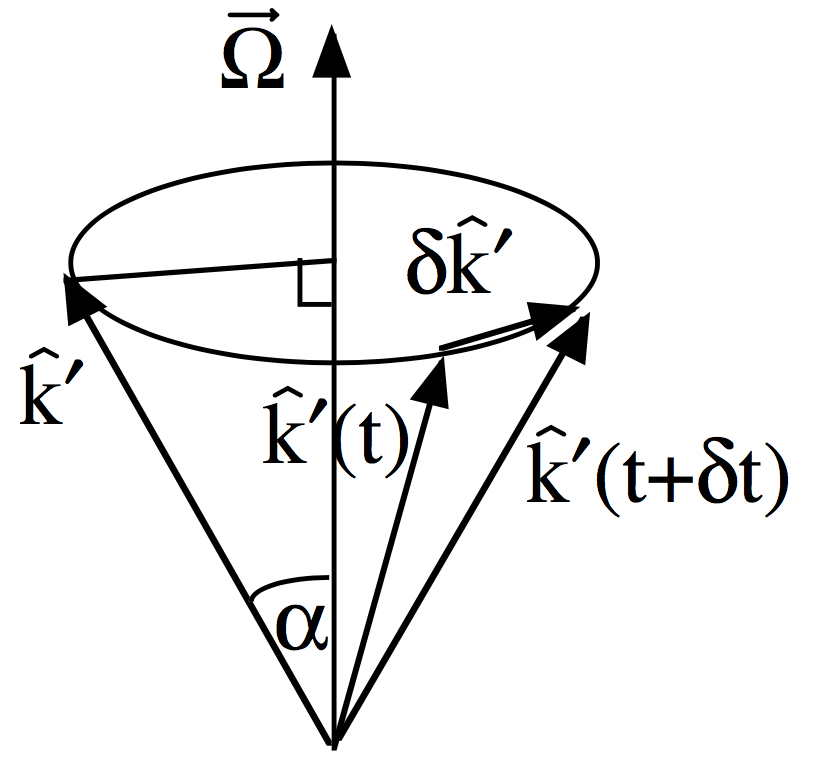
\includegraphics[width=0.4\textwidth]{rotate1.png}
	\end{figure}
	\item tip of $\hat k^\prime (t)$ traces out a circle, $\alpha$ is the angle between $\vv{\Omega}$ and $\hat k^\prime(t)$, and the radius of the circle = $|\hat k^\prime| \sin \alpha = \sin \alpha$.
	\item $\delta \hat k^\prime \equiv \hat k^\prime(t+\delta t) - \hat k^\prime(t)$ is the change in $\hat k^\prime$ over a small time interval  $\delta t$.
\end{itemize}
\end{frame}
%------------------------------------------------
\begin{frame}{Conservation of Momentum: Rotating Coordinate System}
\begin{itemize}
	\item Let's look at the plane perpendicular to the $\vv{\Omega}$ axis
	\begin{figure}
		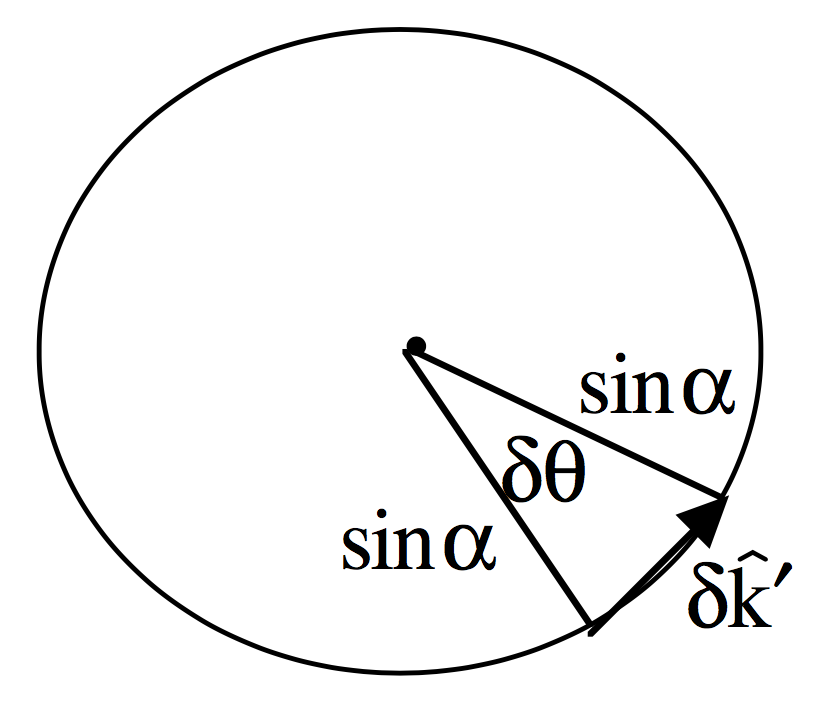
\includegraphics[width=0.3\textwidth]{rotate2.png}
	\end{figure}
	\item $\vv{\Omega}$ is directed out of the center of the cirle and $|\delta \hat k^\prime| = \sin \alpha \delta \theta$.
	$$\left|\frac{D_a \hat k^\prime}{Dt}\right| = \lim_{\delta t\rightarrow 0} \frac{\left|\delta \hat k^\prime\right|}{\delta t} = \lim_{\delta t\rightarrow 0}\sin \alpha \frac{\delta \theta}{\delta t} = \Omega \sin \alpha$$
	But $\left| \vv{\Omega} \times \hat k^\prime \right| = \left| \vv{\Omega}\right| \left| \hat k^\prime \right| \sin \alpha$, so $\left|\frac{D_a \hat k^\prime}{Dt}\right| = \left| \vv{\Omega} \times \hat k^\prime \right|$
\end{itemize}
\end{frame}
%------------------------------------------------
\begin{frame}{Conservation of Momentum: Rotating Coordinate System}
\begin{itemize}
	\item $D_a\hat k^\prime / Dt$ has direction of $\delta \hat k^\prime$ as $\delta t\rightarrow 0$
	\item $\delta \hat k^\prime$ has direction of $\vv{\Omega} \times \hat k^\prime$ ($\delta \hat k^\prime$ is perpendicular to $\vv{\Omega}$ and perpendicular to $\hat k^\prime$ and points in the direction of increasing $\theta$)
	\item Thus, $D_a\hat k^\prime / Dt$ has direction $\vv{\Omega} \times \hat k^\prime$
	\item Since $D_a\hat k^\prime / Dt$ has the same magnitude and direction as $\vv{\Omega} \times \hat k^\prime$, it must be $\vv{\Omega} \times \hat k^\prime$
	\item Thus
	$$\frac{D_a \hat k^\prime}{Dt} = \vv{\Omega} \times \hat k^\prime$$
	and similarly,
	$$\frac{D_a \hat i^\prime}{Dt} = \vv{\Omega} \times \hat i^\prime \qquad \text{and} \qquad \frac{D_a \hat j^\prime}{Dt} = \vv{\Omega} \times \hat j^\prime$$
\end{itemize}
\end{frame}
%------------------------------------------------
\begin{frame}{Conservation of Momentum: Rotating Coordinate System}
\begin{itemize}
	\item We can now write our expression as:
	\begin{align*}
	\frac{D_a\vv{A}}{Dt} &= \frac{D\vv{A}}{Dt} + A_x^\prime \vv{\Omega} \times \hat i^\prime +A_y^\prime \vv{\Omega} \times \hat j^\prime +A_z^\prime \vv{\Omega} \times \hat k^\prime\\
	\frac{D_a\vv{A}}{Dt} &= \frac{D\vv{A}}{Dt} + \vv{\Omega} \times \left(A_x^\prime \hat i^\prime + A_y^\prime \hat j^\prime + A_z^\prime \hat k^\prime\right)\\
	\Aboxed{\frac{D_a\vv{A}}{Dt} &= \frac{D\vv{A}}{Dt} + \vv{\Omega} \times \vv{A}}
	\end{align*}
	\item In words, this says that the total derivative as observed in a non-rotating reference frame is equal to the total derivative as observed in a rotating reference frame plus the apparent force arising from rotation.
\end{itemize}
\end{frame}
%------------------------------------------------
\begin{frame}{Conservation of Momentum: Rotating Coordinate System}
\begin{itemize}
	\item Let's consider the vector form of $\vv{F} = m\vv{a}$, or $\vv{a} = \vv{F} /m$, which holds for an inertial reference frame.
	\item $\vv{a}$ is the acceleration observed in an inertial reference frame:
	$$\vv{a} = \frac{D_a \vv{U}_a}{Dt}$$
	where $\vv{U}_a = D_a \vv{r}/Dt$ is the absolute velocity of an air parcel and $\vv{r}$ is the position vector.
	\item Now we apply the previous relationship and set $\vv{A}=\vv{r}$
	\begin{align*}
		\frac{D_a \vv{r}}{Dt} &= \frac{D\vv{r}}{Dt} + \vv{\Omega} \times \vv{r}\\
		\vv{U}_a &= \underbrace{\vv{U}}_{\text{I}} + \underbrace{\vv{\Omega} \times \vv{r}}_{\text{II}}
	\end{align*}
	where (I) is the relative velocity of the air parcel and (II) is the velocity of solid-body rotation at location $\vv{r}$.so
\end{itemize}
\end{frame}
%------------------------------------------------
\begin{frame}{Conservation of Momentum: Rotating Coordinate System}
\begin{itemize}
	\item Now let's set $\vv{A} = \vv{U}_a$:
	\begin{align*}
		\frac{D_a \vv{U}_a}{Dt} &= \frac{D\vv{U}_a}{Dt} + \vv{\Omega} \times \vv{U}_a\\
		&= \frac{D}{Dt}\left(\vv{U} + \vv{\Omega} \times \vv{r}\right) + \vv{\Omega} \times \left(\vv{\Omega} \times \vv{r}\right)\\
		&= \frac{D\vv{U}}{Dt} + \vv{\Omega}\times\underbrace{\frac{D\vv{r}}{Dt}}_{\vv{U}} + \vv{\Omega} \times \vv{U} + \underbrace{\vv{\Omega}\times \left(\vv{\Omega} \times \vv{r}\right)}_{-\Omega^2\vv{R}}
	\end{align*}
	\begin{figure}
		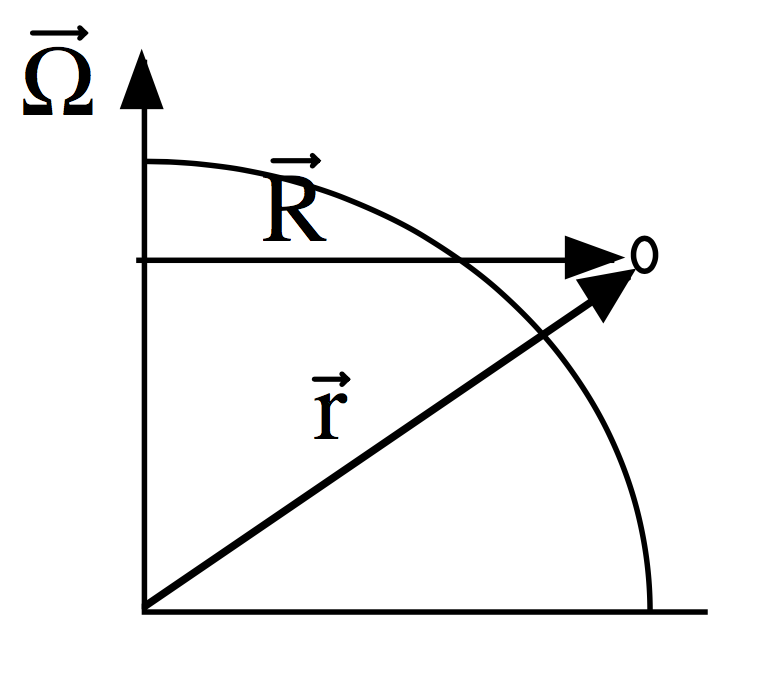
\includegraphics[width=0.3\textwidth]{rotate3.png}	
	\end{figure}
\end{itemize}
\end{frame}
%------------------------------------------------
\begin{frame}{Conservation of Momentum: Rotating Coordinate System}
\begin{itemize}
	\item The final form:
	$$\underbrace{\frac{D_a \vv{U}_a}{Dt}}_{1} = \underbrace{\frac{D\vv{U}}{Dt}}_{2} + \underbrace{\vphantom{\frac{D\vv{U}}{Dt}}2\vv{\Omega}\times \vv{U}}_{3} - \underbrace{\vphantom{\frac{D\vv{U}}{Dt}}\Omega^2 \vv{R}}_{4}$$
\end{itemize}
\begin{enumerate}
	\item acceleration in an inertial reference frame
	\item acceleration in a non-inertial reference frame
	\item Coriolis acceleration
	\item centripetal acceleration
\end{enumerate}
\end{frame}
%------------------------------------------------
\begin{frame}{Conservation of Momentum: Rotating Coordinate System}
\begin{itemize}
	\item Plus this into Newton's \nth{2} Law:
	\begin{align*}
	\frac{D_a\vv{U}_a}{Dt} &= \frac{\vv{F}}{m}\\	
	\frac{D\vv{U}}{Dt} + 2\vv{\Omega}\times \vv{U} -\Omega^2 \vv{R} &= \frac{\vv{F}}{m}
	\end{align*}
	\item Recall that $\vv{F}/m$ is the sum of all the fundamental forces per unit mass
	\begin{itemize}
		\item PGF: $-\frac{1}{\rho}\vv{\nabla}p$
		\item friction: $\nu \vv{\nabla}^2 \vv{U}$
		\item gravitational: $\vv{g^*}$
	\end{itemize}
\end{itemize}
\end{frame}
%------------------------------------------------
\begin{frame}{Conservation of Momentum: Rotating Coordinate System}
\begin{itemize}
	\item Newton's \nth{2} Law becomes:
	\begin{align*}
	\frac{D\vv{U}}{Dt} + 2\vv{\Omega}\times \vv{U} -\Omega^2 \vv{R} = -\frac{1}{\rho}\vv{\nabla}p + \vv{g^*} + \nu \vv{\nabla}^2 \vv{U}\\
	\frac{D\vv{U}}{Dt} = -\frac{1}{\rho}\vv{\nabla}p - 2\vv{\Omega}\times \vv{U} + \underbrace{\vv{g^*} + \Omega^2 \vv{R}}_{\vv{g}}+ \nu \vv{\nabla}^2 \vv{U}
	\end{align*}
	We arrive at the vector equation of motion in a rotating reference frame:
	$$\boxed{\frac{D\vv{U}}{Dt} = -\frac{1}{\rho}\vv{\nabla}p - 2\vv{\Omega}\times \vv{U} + \vv{g} + \nu \vv{\nabla}^2\vv{U}}$$
\end{itemize}
\end{frame}
%------------------------------------------------
\begin{frame}{Conservation of Momentum: Rotating Coordinate System}
$$\boxed{\underbrace{\vphantom{-\frac{1}{\rho}\vv{\nabla}p}\frac{D\vv{U}}{Dt}}_{1} = \underbrace{-\frac{1}{\rho}\vv{\nabla}p}_{2} - \underbrace{\vphantom{-\frac{1}{\rho}\vv{\nabla}p}2\vv{\Omega}\times \vv{U}}_{3} + \underbrace{\vphantom{-\frac{1}{\rho}\vv{\nabla}p}\vv{g}}_{4} + \underbrace{\vphantom{-\frac{1}{\rho}\vv{\nabla}p}\nu \vv{\nabla}^2\vv{U}}_{5}}$$
\begin{enumerate}
	\item acceleration in a rotating reference frame
	\item pressure gradient force
	\item Coriolis force
	\item gravity
	\item friction
\end{enumerate}
\end{frame}
%------------------------------------------------
\end{document}

